\documentclass[11pt]{article}

% Variable for HW number & name:
\newcommand{\class}{Stats 305c}
\newcommand{\hwnum}{2}
\newcommand{\quarter}{Spring 2026}

% Packages
\usepackage[margin=1in]{geometry}             
\geometry{letterpaper}                  
\usepackage{graphicx}
\usepackage{physics}
\usepackage{amsmath, amssymb, amsthm}
\usepackage{hyperref, multicol}
\hypersetup{colorlinks=false, allcolors=blue}
\usepackage[shortlabels]{enumitem}
\usepackage{bbm}
\usepackage{float}

% Commands for distributions
\newcommand{\Bern}{\mathrm{Bern}}
\newcommand{\Bin}{\mathrm{Bin}}
\newcommand{\HGeom}{\mathrm{HGeom}}
\newcommand{\Geom}{\mathrm{Geom}}
\newcommand{\FS}{\mathrm{FS}}
\newcommand{\Pois}{\mathrm{Pois}}
\newcommand{\Unif}{\mathrm{Unif}}
\newcommand{\Expo}{\mathrm{Expo}}
\newcommand{\Beta}{\mathrm{Beta}}
\newcommand{\Gam}{\mathrm{Gamma}}
\newcommand{\Logistic}{\mathrm{Logistic}}
\newcommand{\Nml}{\mathcal{N}}
\newcommand{\Lyap}{\mathrm{Lyap}}
\newcommand{\Lind}{\mathrm{Lind}}
\newcommand{\Rademacher}{\mathrm{Rademacher}}

% Commands for Var, Cov, Cor, etc.
\newcommand{\E}{\mathbb{E}}
\renewcommand{\P}{\mathbb{P}}
\newcommand{\Hcal}{\mathcal{H}}
\newcommand{\Var}{\mathrm{Var}}
\newcommand{\Cov}{\mathrm{Cov}}
\newcommand{\Cor}{\mathrm{Cor}}
\newcommand{\indi}{\mathbbm{1}}

% Commands for convergence
\newcommand{\toprob}{\xrightarrow{P}}
\newcommand{\todist}{\xrightarrow{D}}
\newcommand{\toas}{\xrightarrow{a.s.}}
\newcommand{\tolaw}{\xrightarrow{\mathcal{L}}}

% Commands for mathbb
\newcommand{\R}{\mathbb{R}}
\newcommand{\N}{\mathbb{N}}
\newcommand{\F}{\mathcal{F}}
\newcommand{\Q}{\mathbb{Q}}
\newcommand{\Z}{\mathbb{Z}}
\newcommand{\C}{\mathbb{C}}

% Setup for tcolorbox
\usepackage[most]{tcolorbox}
\tcbset{colback=green!5, colframe=green!75!black}

% Paragraph settings
\setlength{\parindent}{0pt}
\setlength{\parskip}{1.25ex}

% Solution environment
\newenvironment{sol}
    {\begin{tcolorbox}[breakable, pad at break*=1mm, parbox=false]
    }
    {
    \end{tcolorbox}
    }
    
% Page headers
\usepackage{fancyhdr}
\pagestyle{fancy}
\lhead{Kenny Gu and Scott Hwang}
\rhead{\class, Milestone \hwnum}

\newcommand{\noin}{\noindent}

% Indep symbol
\DeclareSymbolFont{symbolsC}{U}{txsyc}{m}{n}
\DeclareMathSymbol{\indep}{\mathrel}{symbolsC}{121}

% Document info
\title{\class\ Milestone \hwnum}
\author{Kenny Gu}
\date{April 2026}
                        
\begin{document}

%\maketitle
%\thispagestyle{empty}
%\newpage
 
% \noindent {\large  \textbf{\class\ Milestone \hwnum, \quarter}}

% \medskip

\newcommand{\KL}{\text{KL}}
\newcommand{\pse}{\tilde{E}}
\newcommand{\Et}{\tilde{E}}
\newcommand{\bm}[1]{\mathbf{#1}}
\renewcommand{\d}{\mathrm{d}}

\textbf{Data description.} We are using data from the Federal Election Commission, which collects and processes mandatory contribution reports from political campaigns. To get a sense of what contributions and the data ``looked like,'' we first looked through the FEC's \href{https://www.fec.gov/data/receipts}{campaign finance data browser}: unfortunately, however, the FEC does not allow us to export more than 500,000 entries at once from the browser, so we must instead download bulk data files. 

In particular, we first choose to browse through bulk data from 2022 for individual contributors, which is distributed as a massive \texttt{.zip} file that is around 5.21 GB in size. When uncompressed, it appears as a \texttt{.txt} file that is about 12.08 GB in size and contains \emph{all} individual contributions (i.e., across races, states, etc.). It is also separately divided into 34 \texttt{.txt} files across time.

We choose (for now) to focus on individual contributions that (a) occur between January 1, 2021 and December 31, 2022, (b) have receipts reported during the 2021-2022 election cycle, (c) are reported as individual contributions, and (d) goes directly to a Senate candidate committee. We use the candidate master and candidate-committee linkage files, in correspondence with the individual contributions files, to filter entries in the bulk data file. There are a total of 63,885,895 entries in the raw data file, and our filtering leaves us with 2,017,528 entries. 

Some of our filtering involves important decisions about our data: receipts are not always reported in a timely manner, so we may be missing some receipts that instead appear in the 2022-2023 election cycle bulk file. However, a cursory look at the 2022-2023 reports on the FEC browser suggests that this is an insignificant amount of receipts. 

When looking at the data, one of the first things we noticed was that there were a fair number of contributions reported as negative numbers. Some searching revealed that these usually appear as refunds for contribution errors. Therefore, we choose to leave these negative numbers in our data for now so that the central summary statistics are accurate. In particular, we find that the mean contribution is \$131.96, while the median is \$25.00, reflecting the fact that contributions have a heavy right tail: in fact, the $75$th percentile is only \$100.00. We also note that there are 1711 contributions of over \$2,900, the FEC individual contribution limit for campaigns: i.e., these campaign contributions were not allowed. We infer that these contributions must have been refunded in some form and thus keep them in our data for now. We note that the analogous data for the 2019-2020 cycle that we mention later in this report follows much of the same patterns.

For election results, we get our data from the FiveThirtyEight \href{https://github.com/fivethirtyeight/election-results/tree/main}{Senate elections result repository}, which compiles data directly from Secretaries of State.

\textbf{Exploratory analysis.} As hinted to earlier, 86\% of contributions are between \$0 and \$200 (non-inclusive), even though the FEC only mandates reports for individuals who have donated at least \$200 in a single cycle (including the current donation). We attribute this to three factors: (1) many campaigns still simply report all/most contributions, even when they are not mandated, (2) many individuals who cross the \$200 threshold do so through several contributions, and (3) many contributions occur through third-party contribution sites (e.g., ActBlue or WinRed), which then tally over the \$200 threshold (as the organization), even though individual contributions through the sites might not tally over \$200. 

We then tally contributions by zip code (noting that 00000 has a total of \$216,783 in contributions, even though the zip codes does not exist --- this is an error in the data!), and we see that the top contributions correspond to Palm Beach, Manhattan, and Montgomery County, which all contain wealthy areas known for large political contributions/involvement. Tallying by state reveals a similar phenomenon, capturing the same general regions: the top states are CA, NY, FL, and TX. We note though that there are two additional effects to consider here: some zip codes/states have bigger/smaller populations, and some states didn't have Senate elections in 2022. 

We can plot the distribution of contributions (a) by individual, (b) for the top 100 zip codes, and (c) for all 50 states: 
\begin{center}
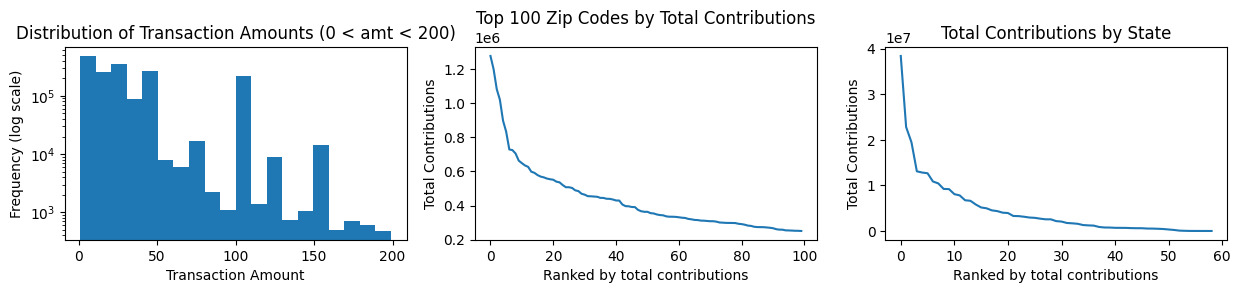
\includegraphics[width=0.8\textwidth]{analysis/figures/transaction_amount_distribution.png}
\end{center}
This analysis motivates us to consider aggregating sums at the zip code level. At the individual level, the distribution of contributions seems almost to drop at a double exponential rate, making it extremely difficult to meaningfully predict contributions. However, at the zip code level, we see a much more steady (albeit still seemingly exponential) dropoff in contributions, which may be much easier to model. A similar result holds for contributions by state, though we believe this level of detail to be too coarse for interesting modeling.

We then decided to repeat the same analysis for the 2020 data, understanding that this data might look different for a few reasons: (1) the POTUS election in 2020 leads to more political participation, (2) COVID may have led to different political involvement, (3) political polarization leads to more involvement, (4) certain states had Senate elections in 2020 but not 2022 (and vice versa). We see that the median contribution decreased by 50\% from the 2020 cycle to the 2022 cycle. We also see that many of the zip codes and states with dramatic changes from one cycle to another have highly contentious Senate elections in one but not the other (e.g., Ohio and Colorado), which highlights reason (4). In general, however, contributions were significantly higher in 2020 than 2022 (median contribution was \$25 higher). We then plot the absolute value of the percent change in campaign contributions against the margin of victory at the state and zip code level, which makes this relationship clearer:

\begin{center}
    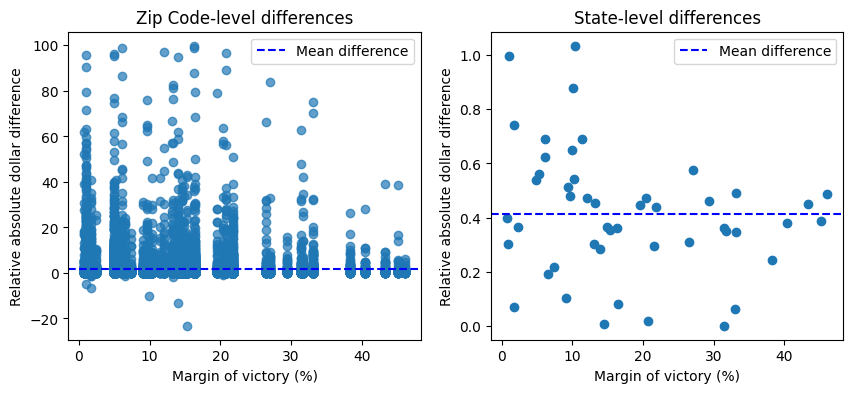
\includegraphics[width=0.8\linewidth]{analysis/figures/margin_vs_diff.png}
\end{center}

\textbf{Refined model sketch.} Based on our analysis, we might choose to predict campaign contributions at the zip code level, modeling idiosyncratic noise as a random surface (i.e., covariance between zipcodes is described by a function of the distance) and modeling the true mean with covariates like polling (as a proxy for not yet available election results), whether a Senate election is taking place in the state, whether a POTUS election is occuring, and donations  from the past cycle. We might hope that the marginal distribution of contributions per zip code is modeled by a Weibull (or something similar), which might accurately capture the general shape of the marginal distribution seen in our visualizations/EDA. 

\newpage
\textbf{AI disclosure.} We used ChatGPT to help us efficiently read in the bulk files, streamline our code for filtering the data, and to format figures (especially the geospatial visualizations). We also used GitHub Copilot inline suggestions throughout the analysis. All code was still scrutinized and checked by us.

\textbf{GitHub repository.} \href{https://github.com/kennethgu/stats305c-project/}{https://github.com/kennethgu/stats305c-project/}

% \bibliographystyle{plain} 
% \bibliography{milestone1}

\end{document}